%    This file is part of BGSU.cls The BGSU (Thesis and Dissertation LaTeX class)
%
%    BGSU.cls is free software: you can redistribute it and/or modify
%    it under the terms of the GNU General Public License as published by
%    the Free Software Foundation, either version 3 of the License, or
%    (at your option) any later version.
%
%    BGSU.cls is distributed in the hope that it will be useful,
%    but WITHOUT ANY WARRANTY; without even the implied warranty of
%    MERCHANTABILITY or FITNESS FOR A PARTICULAR PURPOSE.  See the
%    GNU General Public License for more details.
%
%    You should have received a copy of the GNU General Public License
%    along with BGSU.cls  If not, see <http://www.gnu.org/licenses/>.
%
%    Note that this only applies to the example and template files and BGSU.cls
%    itself. Any actual document content (such as your thesis or dissertation text)
%    belongs solely to you and you can do with it what you please.

\documentclass{BGSU}

% For thesis, open BGSU.cls and change line 57 to \def\@doctype{Thesis}

\usepackage{amsmath}
\usepackage{amssymb}   % allows the use of AMS symbols like blackboard bold
\usepackage{graphicx}
\usepackage{caption}
\usepackage{amsthm}    % allows AMS definitions for theorems, proofs, etc.
\usepackage{epstopdf}
\usepackage{times}     % Times New Roman (nimbus version)
\usepackage{listings}  % allows program codes embeded with original forms
\usepackage{bookmark}  % make it possible to add PDF bookmarks at will
\usepackage{pdflscape} % make it possible to use landscape environment
\usepackage[nottoc,notlof,notlot]{tocbibind} % keep list of figures, tables, out of the table of contents, also keep the table of contents out of the table of contents
\usepackage[longnamesfirst]{natbib} %You need to insert comment (%) if you don't want to use natbib for bibliography


\newtheorem{theorem}{\bf Theorem}[chapter]         % Allow numbered theorems
\newtheorem{proposition}[theorem]{\bf Proposition} % Number props with theorems
\newtheorem{remark}[theorem]{\bf Remark}           % Number remarks too
\newtheorem{lemma}{Lemma}[chapter]
\numberwithin{equation}{chapter}
\setcounter{equation}{0}


% Change the text below -----------------------------------------------

\title{An example dissertation}
\author{Nate Iverson}
\degree{Doctor of Philosophy}
\date{August 2007}
\advisor{Corneliu Hoffman}
\gfr{Darth Vader} % graduate faculty representative
\committee{Kit Chan \\ \\ Warren McGovern}

\begin{document}

\frontmatter % makes page #'s lower case roman

\maketitle

\copyrightpage % copyrighting your dissertation is optional

\begin{abstract}

















\end{abstract}

% optional section ``Some students choose to personalize their manuscripts
% with an appropriate quotation or illustration''
% formatting and placement is up to you.
\begin{dedication}
% This text is automatically centered left and right on the page
I would like to dedicate this work to the memory of my grandparents.
They were a great inspiration to me.
\end{dedication}

% optional but encouraged section ``as a means to recognize and express
% appreciation to the people who were influential in preparing and completing
% the manuscript''
\begin{acknowledgments}
Text of acknowledgments goes here.





\end{acknowledgments}

\pdfbookmark[section]{\contentsname}{toc}  % put toc in PDF bookmarks
\tableofcontents

\listoffigures
\pagebreak
\listoftables

% preface section is optional
\begin{preface}
\thispagestyle{myheadings}
Blah Blah Blah...
\end{preface}

\mainmatter % starts over page counter and gives regular page numbers

\setcounter{equation}{0} \numberwithin{equation}{section}

\section{Thoreau}
You never gain something but that you lose something.\\
		-- Thoreau
\section{Unknown}
And dropping a barbell he points to the sky\\

\begin{figure}[h]
\centering
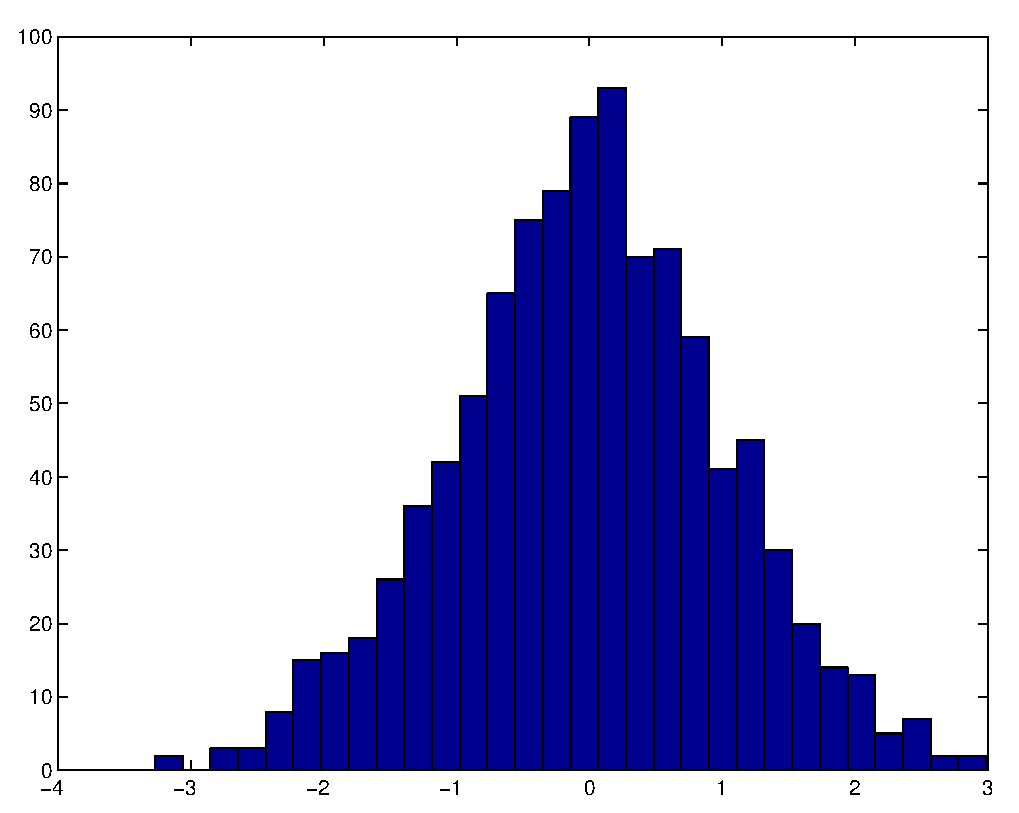
\includegraphics[width = 4.5 in ]{figure.eps}
\caption{Caption of a figure.}\label{FigureLabel}
\end{figure}

\begin{table}[h]
\centering \caption{The values of test
statistics and the corresponding critical values
at~$t_0.$~~$\alpha=0.1.$~}\label{stanford}\vskip .1in
\begin{tabular}{|c|c|c|c|c|c|c|}\hline
$t_0$ & 30 & 60 & 90 & 120 & 150 & 180 \\ \hline
Critical Value & 11.2282 & 10.5357 & 11.1108 & 11.7942 & 11.7343 & 11.7471\\ \hline
Test Statistic & 25.3182 & 24.6395 & 24.6049 & 25.6623 & 27.1320 & 29.3247\\ \hline
\end{tabular}
\end{table}

\section{Citations}

%If you use the package natbib for citations, here is the example how to cite an article.
%Many thanks to Dr. Maria Rizzo who worked this section.

To cite an article use cite, citet, or citep.

For ``in text'' citations use citet:  The original result is attributed to \citet{vn28}.
Refer to \citet{mardia70} for an example.
Refer to \cite{mardia70} for an example.

For a ``parenthetical citation'' use citep:  The computations were implemented in R \citep{R}
using bootstrap \citep{dh97,et93}.

When citing a book, it is helpful to mention where to find the result by indicating
a chapter or a page number or an equation number:  \citet[Ch.~6]{et93} discuss additional results.

Add your reference information to the file reference.bib.
Every time you edit reference.bib, run BibTeX on the dissertation.tex file so that LaTeX will know what the references are.

%If you don't want to use natbib, you should insert comment (\%) in the above part.  
%Here is the example to cite an article without using natbib package. \cite{forina1991class}


\begin{sidewaysfigure}[p!]
\centering
{bf Landscape figure}
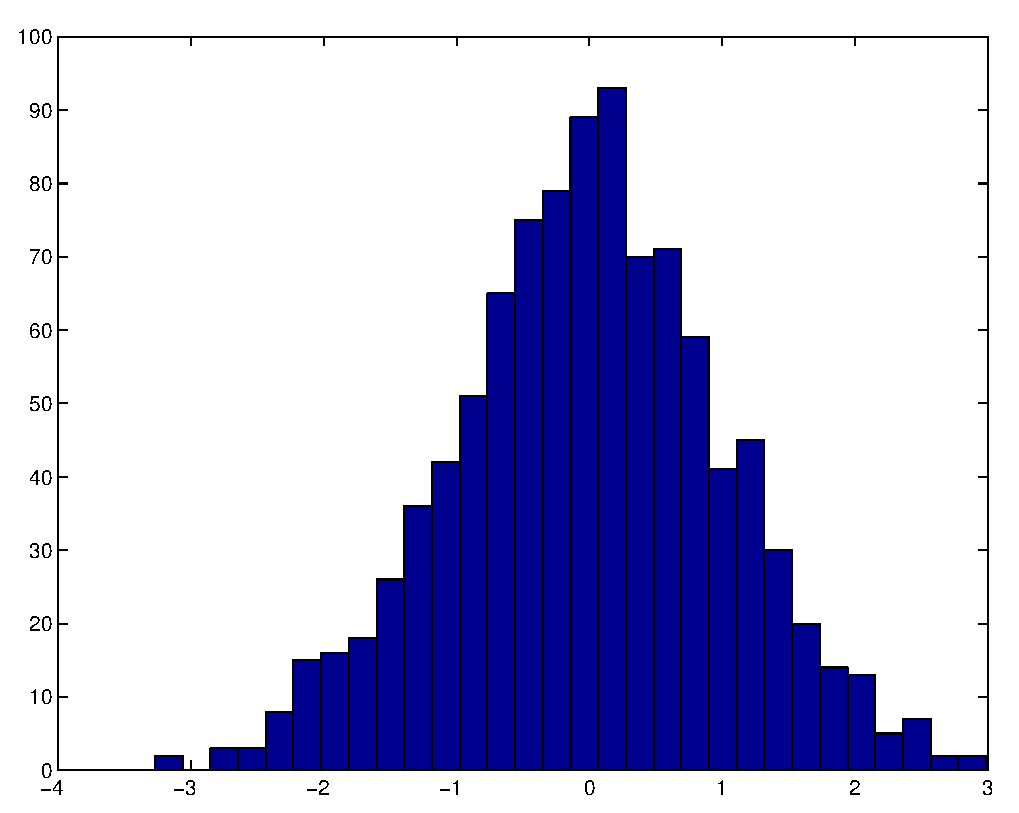
\includegraphics[width=\hsize-1in]{figure.eps}
\caption[Short label for List of Figures]{ 
Long label for under the actual figure.}
\end{sidewaysfigure}



\begin{landscape}
\thispagestyle{lscape}
\pagestyle{lscape}
  \begin{figure}
    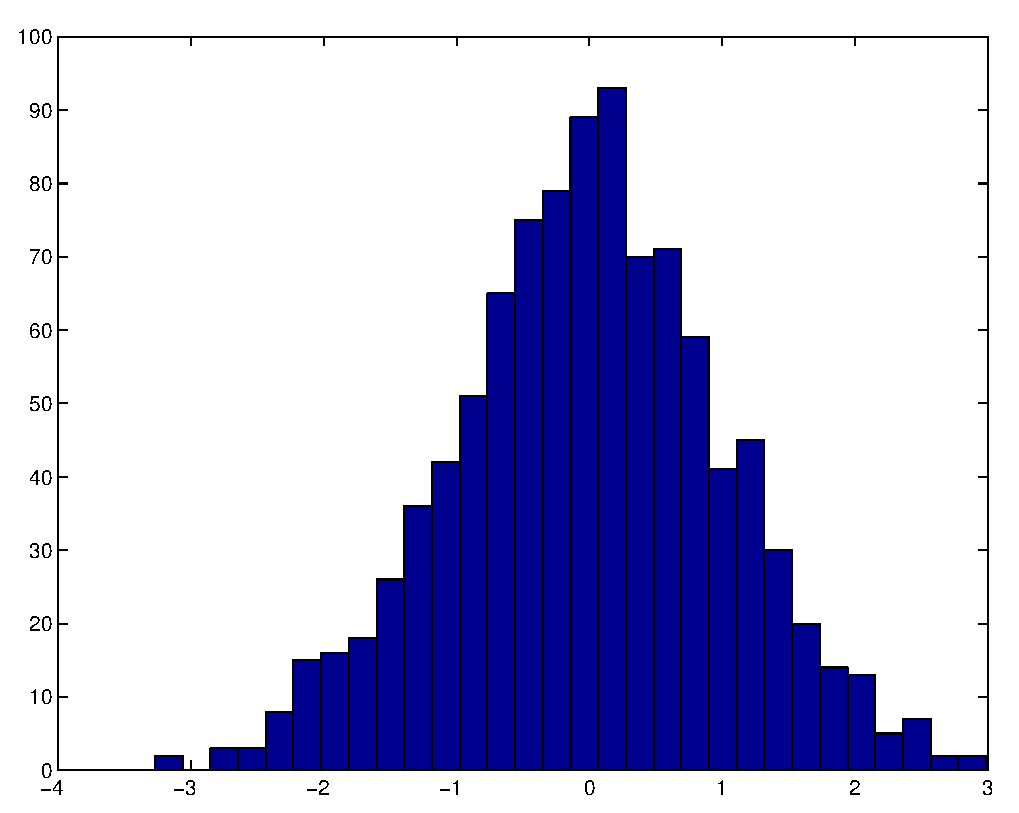
\includegraphics[width=\linewidth,height=\textheight-1in]{figure.eps}
    \caption[Short caption for List of Figures]{Long caption to appear under the figure.  Hopefully the figure is not so large that there is no room for the caption, because then the caption might move to a different page, or the text might go into the margin, and that would be bad!}
  \end{figure}
\end{landscape}

\setcounter{equation}{0} \numberwithin{equation}{section} 

John the Baptist after poisoning a thief,
Looks up at his hero, the Commander-in-Chief,
Saying tell me great leader, but please make it brief
Is there a hole for me to get sick in?
 The Commander-in-Chief answers him while chasing a fly,
Saying death to all those who would whimper and cry.
And dropping a barbell he points to the sky,
Saying the sun is not yellow, it's chicken.
		-- Bob Dylan, "Tombstone Blues"


\setcounter{equation}{0} \numberwithin{equation}{section}
\chapter{\texorpdfstring{HOW TO PROVE IT}{}} %upper case only
\setcounter{equation}{0} 
\numberwithin{equation}{section}

\section{proof by accumulated evidence:}

	Long and diligent search has not revealed a counterexample.

\section{proof by cosmology:}

	The negation of the proposition is unimaginable or
	meaningless. Popular for proofs of the existence of God.

\section{proof by mutual reference:}

	In reference A, Theorem 5 is said to follow from Theorem 3 in
	reference B, which is shown to follow from Corollary 6.2 in
	reference C, which is an easy consequence of Theorem 5 in
	reference A.

\section{proof by metaproof:}

	A method is given to construct the desired proof. The
	correctness of the method is proved by any of these
	techniques.

\chapter{\texorpdfstring{OTHERNESS}{}} %upper case only
\setcounter{equation}{0} 
\numberwithin{equation}{section}

In a surprise raid last night, federal agents ransacked a house in search
of a rebel computer hacker.  However, they were unable to complete the arrest
because the warrant was made out in the name of Don Provan, while the only
person in the house was named don provan.  Proving, once again, that Unix is
superior to Tops10.

\section{deja-vu}

Over the years, I've developed my sense of deja vu so acutely that now
I can remember things that *have* happened before ...

\section{More references}

Once again, we can refer back to Equation \ref{PythagoreanTheorem}.
We can also refer to Equation \ref{squarebinomial}.
Finally, we can refer back to Section \ref{AdditionalNumberedResults}.







\backmatter

%bibliography section: there are two options here. 1. Uncomment the following codes and use \bibitem{} to add more articles.
%\begin{thebibliography}{99}
%\bibitem{forina1991class} Forina, M., Armanino, C., Leardi, R., and Drava, G. (1991). A class-modelling technique based on potential functions. \textit{Journal of Chemometrics,} {\textbf{5(5)},} 435-453.
%\end{thebibliography}

%2. Using natbib package (you may use other bibliography types). Refer to http://en.wikibooks.org/wiki/LaTeX/Bibliography_Management
\bibliographystyle{chicago}    %% this one looks best
%\bibliographystyle{apalike}   %% looks okay for dissertations but it puts quotes around titles in references
\setcitestyle{authoryear, open={((},close={))}}
\bibliography{reference}

% appendix section: if you have more than one appendix section, you should use APPENDIX A, APPENDIX B, ....
\mbox{}\newpage
\phantomsection
\appendix
\chapter{\texorpdfstring{APPENDIX A\hspace{1em}SELECTED R PROGRAMS}{APPENDIX A}}

Text of appendix goes here.

% If you want to put program codes in the appendix, here is one example. 
\begin{itemize}
\item The function kernel is used to compute the kernel function of variances
{\small
\begin{lstlisting}
kernel<-function(x,y){
  h <- 0.5*(x-y)^2
  return(h)
}
\end{lstlisting}
}
\end{itemize}

\end{document}
